\documentclass[a4paper,12pt,oneside]{scrartcl}
\usepackage[utf8]{inputenc}
\usepackage[ngerman]{babel}
\usepackage{hyperref}
\usepackage{graphicx}
\usepackage[section]{placeins}


\title{Gruppe E Lastenheft V0.4}

\begin{document}
\maketitle
\newpage
\tableofcontents
\newpage

\section{Auftraggeber}
Eine Gruppe von vier Master-Studenten der FH Aachen aus dem Studiengang „Information System Engineering“ ist Auftraggeber der Software „Unsocial Selling App“. 




\section{Zeit- und Budgetrahmen}
Die Software „Unsocial Selling App“ wird im Rahmen der Lehrveranstaltung „Software Engineering“ im Fachsemester 5 Studiengang “Angewandte Informatik” an der Fachhochschule Aachen erstellt.
Durch die vorgegebenen ECTS-Punkte für das Praktikum (3 ECTS-Punkte) ist bereits der zeitliche Rahmen vorgegeben.
Daraus ergibt sich eine Arbeitszeit von 156 Stunden pro Person. Insgesamt werden 1248 Zeitstunden für das Projekt vorausgesetzt. 
Davon werden wir 288 Stunden für die Vorbereitung, 480 Stunden für die Planung und 480 Stunden für die Implementierung veranschlagen. 
Am 21.10.2015 fand das erste Gespräch mit dem Auftraggeber statt.
Die erste Release-Version der Software soll am 08.01.2016 an den Kunden übergeben werden.
Die finale Version muss am 15.01.2016 dem Kunden vorliegen und bereit sein für die Vorführung. 




\section{Zielbestimmung}
\subsection{Zweck}
Die Software „Unsocial Selling App“ erlaubt die Kontaktaufnahme zwischen Verkäufern und Kunden.
Dazu bietet sie Verkäufern die Möglichkeit, Annoncen für Produkten und das Anbieten von Dienstleitungen, in einem bestimmten Gebiet und zu einer bestimmten Kategorie, zu erstellen.
Des weiteren können Kunden jene Annoncen sehen, die der Kategorie ihrer Filterliste entsprechen und sich in ihrem Gebiet befinden.
Annoncen von sogenannter Premiumverkäufer, werden dabei häufiger Angezeigt.

\subsection{Nutzen}
„Unsocial Selling App“ bietet den Nutzern die Möglichkeit für schnelles und problemloses impulsiv Einkaufen.
Die Käufer können die Anzeigen nach ihren Interessen filtern.
Dafür wird eine Datenbank verwendet, in der die Angebote der Verkäufer gespeichert werden.
Bei Kaufinteresse bekommt Benutzer Kontaktdaten des Verkäufers.
Durch das Zusammenspiel vieler Nutzer, soll daraus ein schnell Kaufs/Verkaufs App werden.
So hat der Nutzer einerseits die Möglichkeit neue Anzeigen zu erstellen und somit seine Ware schnell verkaufen oder Dienstleistung schnell erbringen.
Andererseits kann er die Waren und Dienstleistungen anderer Nutzern schnell bekommen.




\section{Produckteinsatz}
\subsection{Anwendungsbereich}
Der Benutzer muss:
\begin{itemize}
	\item die Software starten können 
	\item Nach dem Start die Startseite mit einer Anzeige, sowie deren Bild und Namen angezeigt werden 
	\item auf der Startseite ein Menü auswählen können, über welches er sich einloggen oder registrieren kann 
	\item die Möglichkeit haben, sein Passwort zurückzusetzen 
	\item eine Anzeige ablehnen können 
	\item vorgegebene Kategorien einfügen können, welche die Anzeigenmenge filtert 
	\item eine Detailansicht der Anzeige aufrufen können, welche weitere Bilder, Preis, Entfernung und Beschreibung in Form eines Textes darstellt 

	\item sofern er eingeloggt ist: 
	\begin{itemize}
		\item dem Anbieter, via Detailansicht der Anzeige, sein Interesse bekunden können
		\item eine Anzeige einstellen könne	
	\end{itemize}
\end{itemize}

\begin{figure}[!htbp]
\centering
\noindent
\includegraphics[width=\linewidth,height=\textheight,keepaspectratio]{Diagramme/Anwendungsbereiche}
\caption{Use-Case Diagramm Anwendugsbereiche}
\end{figure}
\FloatBarrier


\subsection{Zielgruppe und Anwender}
Die Software „Unsocial Selling App“ richtet sich an Menschen, die auf schnelle und unkomplizierte Weise Produkte und Dienstleistungen erwerben möchten.
Bei bekannten Verkaufsplattformen im Internet ist das Stöbern oft sehr unübersichtlich.
Die Software „Unsocial Selling App“ hingegen überzeugt durch ein besonders simples Bedienkonzept und ist somit für alle Personen, die gerne online einkaufen, geeignet.


\subsection{IST-Prozesse}
Aktuell gibt es nur Verkaufsplattformen, die den Benutzer nach konkreten Produkten suchen lassen ihn aber nicht mit zufälligen Vorschlägen überraschen.
Auch steht der Impulskauf bei diesen Plattformen nicht im Fokus, sodass der Kunde auch vorher gesichtete Produkte später noch einmal aufrufen kann. 


\subsection{Unterstützte SOLL-Prozesse}
Die Software muss folgende Funktionen zur Verfügung stellen:
\begin{itemize}
	\item Registrierung und Benutzerlogin
	\item Für eingeloggte Benutzer:
	\begin{enumerate}
		\item Verwaltung des Profils
		\item Erstellen neuer Anzeigen
	\end{enumerate}
	\item Für eingeloggte und nicht eingeloggte Benutzer:
	\begin{enumerate}
		\item Filterung der Anzeigen nach Kategorien und Standort
		\item Aufrufen der Detailansicht einer Anzeige
		\item Ablehnen eines Angebotes um Neues zu erhalten
	\end{enumerate}
	\item Premiumverkäufer, dessen Annoncen priorisiert behandelt werden
\end{itemize}




\section{Produktfunktionen}
\subsection{Alle Funktionen, Eingabe/Ausgabe, beschrieben aus Anwendersicht}

\subsubsection*{Anmerkung:}
Einige Buttons können je nach Implementation für ein bestimmtes Betriebssystem wegfallen und durch Swipe-Gesten ersetzt werden.
Die Funktionalität muss jedoch erhalten bleiben.


\subsubsection{Aktivität u00 - Starten der Software}
Während des Startvorgangs muss dem Benutzer eine Warteanzeige angezeigt werden.
Sollte der Start nicht erfolgreich verlaufen, muss dem Benutzer eine Fehlermeldung angezeigt werden.
Ist der Start hingegen erfolgreich, muss dem Benutzer die Hauptseite angezeigt werden.

\begin{figure}[!htbp]
\centering
\noindent
\includegraphics[width=\linewidth,height=\textheight,keepaspectratio]{Diagramme/Aktivitaet_u00}
\caption{Starten der Software}
\end{figure}
\FloatBarrier


\hypertarget{u01}{\subsubsection{Aktivität u01 – Startbildschirm}}
Nach erfolgreichem Starten der Software muss dem Benutzer die Startseite angezeigt werden. 
Auf der Startseite müssen folgende Informationen angezeigt werden:
\begin{itemize}
	\item Eine Annonce mit einem Namen, der aus maximal 100 Zeichen bestehen darf
	\item Ein Button, der ein Angebot ablehnt und somit Desinteresse zeigt
	\item Ein Bild der Annonce, welches beim Drücken zur Detailansicht führt
	\item Der Preis des Angebotes
	\item Eine Navigationsleiste mit Button, welcher das Menü aufruft
\end{itemize}
Das Hauptmenü muss folgende Menüpunkte beinhalten:
\begin{itemize}
	\item Startbildschirm
	\item zustandsabhängige Anzeige
	\begin{itemize}
		\item falls angemeldet: Ausloggen 
		\item falls nicht angemeldet: Einloggen 
	\end{itemize}
	\item Registrieren
	\item Einstellungen:
	\begin{itemize}
		\item Passwort des Benutzers ändern
		\item Filterung
	\end{itemize}
	\item Annonce einstellen
\end{itemize}

Der Menübutton befindet sich oben rechts.
Der Button zum Ablehnen eines Angebots muss sich unten rechts befinden und der Button für die Detailansicht unten links.
Es müssen Swipe-Gesten auf das Startbild der Anzeige möglich sein, um die aktuelle Anzeige zu verwerfen und die nächste Anzeige darzustellen.
Entsprechende Buttons entfallen in diesem Fall.

\begin{figure}[!htbp]
\centering
\noindent
\includegraphics[width=\linewidth,height=\textheight,keepaspectratio]{Diagramme/Aktivitaet_u01}
\caption{Startbildschirm}
\end{figure}
\FloatBarrier


\hypertarget{u02}{\subsubsection{Aktivität u02 - Detailansicht}}
In der Detailansicht eines Angebots müssen dem Benutzer folgende Details angezeigt werden:
\begin{itemize}
	\item Preis
	\item 0-10 Bilder des Angebots
	\item (Modular designbare Elemente)
	\item Angebotsbeschreibung (bis zu [X] Zeichen)
	\item Entfernung vom Standpunkt des Benutzers zum Angebot
\end{itemize}
Der Benutzer muss das Angebot ablehnen können oder dem Verkäufer sein Interesse melden können.
Dies muss über zwei Buttons realisiert werden.
Der Button zum Ablehnen eines Angebots muss sich unten rechts befinden und der Button, der Interesse bekundet, muss sich unten links befinden.
Nachdem der Benutzer Interesse gemeldet hat, muss ein Pop-Up mit den Kontaktdaten des Verkäufers  erscheinen und es muss der Interessenliste hinzugefügt werden.
Das Pop-Up-Fenster muss einen „OK“-Button enthalten, mit dem der Benutzer wieder auf die Startseite geleitet wird.

\begin{figure}[!htbp]
\centering
\noindent
\includegraphics[width=\linewidth,height=\textheight,keepaspectratio]{Diagramme/Aktivitaet_u02}
\caption{Detailansicht eines Angebots}
\end{figure}
\FloatBarrier


\subsubsection{Aktivität u03 – Einloggen}
Über den Menübutton muss der Benutzer die Möglichkeit haben, auf einen Eintrag „Einloggen“ klicken zu können.
Anschließend muss dem Benutzer eine Seite angezeigt werden, auf der der Benutzer sich mit seiner E-Mail-Adresse und seinem Passwort einloggen können muss.
Der Benutzer muss außerdem die Möglichkeit haben, auf eine Schaltfläche „Passwort vergessen“ klicken zu können. Mit dieser Schaltfläche muss der Benutzer sein Passwort zurücksetzen können.
Ist eine korrekte E-Mail-Adresse im Login-Feld eingegeben, so muss an diese E-Mail-Adresse eine E-Mail geschickt werden, die ein neues Passwort des Benutzers beinhaltet.
Gibt der Benutzer bei einem Loginversuch eine falsche E-Mail-Adresse oder ein falsches Passwort zu einer korrekten E-Mail-Adresse ein, so muss ihm eine Fehlermeldung angezeigt werden.
Hat der Benutzer seine Daten korrekt eingegeben und auf den Button „Einloggen“ geklickt, so muss er zurückgeleitet werden auf die Seite, von der aus er die Einloggen-Aktivität gestartet hat.

\begin{figure}[!htbp]
\centering
\noindent
\includegraphics[width=\linewidth,height=\textheight,keepaspectratio]{Diagramme/Aktivitaet_u03}
\caption{Einloggen}
\end{figure}
\FloatBarrier


\subsubsection{Aktivität u04 – Registrierung}
Über den Menübutton muss der Benutzer die Möglichkeit haben, einen Eintrag „Registrieren“ auszuwählen.
Anschließend muss dem Benutzer ein Formular zur Registrierung angezeigt werden, in das der Benutzer seine Daten eintragen können muss.
Ein Button „Registrierung abschließen“ muss die Daten an das System leiten, welches die Korrektheit der Daten überprüfen muss.
Das System muss prüfen, dass die E-Mail-Adresse noch nicht vorhanden ist, dass es sich dabei um eine valide E-Mailadresse handelt und ob der Benutzer das Passwort zweimal identisch eingegeben hat.
Ist die E-Mail noch nicht vorhanden und die Passwörter identisch, so müssen die neuen Benutzerdaten in der Datenbank gespeichert werden. Anschließend wird der Registrierungsdialog geschlossen und der Benutzer befindet sich wieder auf der Seite, von der aus er die Einloggen-Aktivität gestartet hat.
Außerdem muss der registrierte Benutzer nun auch eingeloggt sein.
Zur Registrierung müssen folgende Daten vom Benutzer eingegeben werden:
\begin{itemize}
	\item E-Mail-Adresse
	\item Passwort (muss in zwei Felder eingegeben werden zur Überprüfung)
\end{itemize}

\begin{figure}[!htbp]
\centering
\noindent
\includegraphics[width=\linewidth,height=\textheight,keepaspectratio]{Diagramme/Aktivitaet_u04}
\caption{Registrierung}
\end{figure}
\FloatBarrier
Es muss außerdem ein Hinweis angezeigt werden, dass der Benutzer zur Registrierung volljährig sein muss.


\subsubsection{Aktivität u05 - [Platzhalter]}


%\subsubsection{Aktivität u05 – Artikel ablehnen}
%Der Benutzer muss auf dem Startbildschirm und in der Detailansicht einen Artikel ablehnen können, der ihm nicht gefällt. Dieser Artikel darf dem Benutzer nicht wieder angezeigt werden.
%Siehe \hyperlink{u01}{Aktivität u01} und \hyperlink{u05}{Aktivität u05}.
%
%\hypertarget{u05}{\subsubsection{Aktivität u05 – Detailansicht}}
%In der Detailansicht eines Artikel müssen dem Benutzer folgende Details eines Artikels angezeigt werden:
%\begin{itemize}
%	\item Artikelname (bis zu 100 Zeichen)
%	\item Artikelpreis
%	\item 1-3 Bilder des Artikels
%	\item Artikelbeschreibung (bis zu [X] Zeichen)
%	\item Entfernung vom Standpunkt des Benutzers zum Artikel
%\end{itemize}
%Der Benutzer muss den Artikel ablehnen können oder dem Verkäufer sein Interesse melden können. Dies muss über zwei Buttons realisiert werden. Der Button zum Ablehnen eines Artikels muss sich unten rechts befinden und der Button, der Interesse bekundet, muss sich unten links befinden.
%Nachdem der Benutzer Interesse gemeldet hat, muss ihn ein Pop-Up darauf hinweisen, dass der Prozess erfolgreich war und dem Verkäufer eine Email geschickt wurde. Das Pop-Up-Fenster muss einen „OK“-Button enthalten, mit dem der Benutzer wieder auf die Startseite geleitet wird.

%\begin{figure}[!htbp]
%\centering
%\noindent\includegraphics[width=\linewidth,height=\textheight,keepaspectratio]{Diagramme/Aktivitaet_u05}
%\caption{Detailansicht eines Artikels}
%\end{figure}
%\FloatBarrier


\subsubsection{Aktivität u06 – Interessen Liste}
Der Benutzer muss die Möglichkeit haben, eine Liste der Angebote aufzurufen, für die er Interesse gemeldet hat (\hyperlink{u02}{a0204}).
Die Interessen Liste muss der Benutzer über das Menü aufrufen können. 
Sollte ein Verkäufer eine Annonce aus der Datenbank entfernen, so darf diese bei keinem Benutzer mehr in der Interessen Liste aufgelistet werden.
Der Benutzer muss ein Angebot aus der Liste auswählen können und das System muss ihm daraufhin erneut die Kontaktdaten des Verkäufers anzeigen.

\begin{figure}[!htbp]
\centering
\noindent\includegraphics[width=\linewidth,height=\textheight,keepaspectratio]{Diagramme/Aktivitaet_u06}
\caption{Interessen Liste}
\end{figure}
\FloatBarrier


\subsubsection{Aktivität u07 – Einstellungen}
Der Benutzer muss über das Menü die Seite „Settings“ aufrufen können.
Auf dieser Seite muss der Benutzer folgende Einstellungen vornehmen können:
\begin{itemize}
	\item Ändern des Benutzerpasswortes (Durch zweimalige Eingabe als Kontrolle)
	\item Filterung der angezeigten Angebote (\hyperlink{u08}{Aktivität u08})
	\item Radius indem sich Angebote befinden können.
\end{itemize}

\begin{figure}[!htbp]
\centering
\noindent\includegraphics[width=\linewidth,height=\textheight,keepaspectratio]{Diagramme/Aktivitaet_u07}
\caption{Einstellungen}
\end{figure}
\FloatBarrier


\hypertarget{u08}{\subsubsection{Aktivität u08 – neue Anzeige einstellen}}
[todo editieren aktivitätsdiagramm, text auf diagramme verteilen, u84 aufteilen]
Der Benutzer muss über den Menüpunkt „my adverts“ auf die Seite gelangen können, auf der seine zum Verkauf angebotenen Produkte und Dienstleistungen dargestellt werden.
Er muss eine neue Anzeige mit der zugehörigen Detailansicht erstellen können.
Hier muss der Benutzer in der Lage sein, eine Anzeige und die dazugehörige Detailansicht zu erstellen.
Bevor das Erstellen vollendet ist, muss der Benutzer ein Titelbild und einen Titeltext bestimmt haben sowie auf der Detailseite einen Ort und Preis angeben, welche der Anzeige zugeordnet werden.
Ebenso muss die Möglichkeit bestehen, den Vorgang des Erstellens zu unterbrechen und zurück auf die Seite „my adverts“ zu gelangen.
Nachdem der Benutzer eine Anzeige erstellt hat, wird die Anzeige in die Datenbank eingefügt.
Anschließend muss der Benutzer zurück auf die Seite „my adverts“ gelangen. 
Bei der Erstellung der Detailansicht für eine neue Anzeige muss der Benutzer aus folgenden dynamischen Elementen frei kombinieren können:

\begin{itemize}
	\item Bildelemente, die das Hochladen von Bildern ermöglichen.
	\item Textelemente, die das Eingeben einer Anzeigenbeschreibung ermöglichen.
	\item Listenelemente, die das Anzeigen von Listen ermöglichen.
\end{itemize}
Dabei muss der Benutzer zwischen 0 und 10 Elementen frei auswählen können.
Ein nachträgliches Ändern oder Löschen der einzelnen Elemente muss während der Erstellung möglich sein.
Das Anordnen der einzelnen Elemente muss in vertikaler Richtung möglich sein und geschieht über Pfeil-Buttons, die oben und unten jeweils mittig auf dem Element liegen.
Ein nachträgliches Löschen ist über einen X-Button möglich, der in der oberen rechten Ecke auf dem Element liegt.

\begin{figure}[!htbp]
\centering
\noindent\includegraphics[width=\linewidth,height=\textheight,keepaspectratio]{Diagramme/Aktivitaet_u08}
\caption{neue Annonce einstellen}
\end{figure}
\FloatBarrier

\begin{figure}[!htbp]
\centering
\noindent\includegraphics[width=\linewidth,height=\textheight,keepaspectratio]{Diagramme/Aktivitaet_u81}
\caption{Menü}
\end{figure}
\FloatBarrier

\begin{figure}[!htbp]
\centering
\noindent\includegraphics[width=\linewidth,height=\textheight,keepaspectratio]{Diagramme/Aktivitaet_u84}
\caption{Menü}
\end{figure}
\FloatBarrier

\begin{figure}[!htbp]
\centering
\noindent\includegraphics[width=\linewidth,height=\textheight,keepaspectratio]{Diagramme/Aktivitaet_u85}
\caption{Menü}
\end{figure}
\FloatBarrier

\subsubsection{Aktivität u09 - [Platzhalter]}

\subsubsection{Aktivität u10 – Menü}
Der Benutzer muss über das Menü:
\begin{enumerate}
	\item „home“ aufrufen können. Das System muss den Benutzer auf die Start-Seite führen.
	\item „settings“ aufrufen können. Das System muss den Benutzer auf die Settings-Seite führen.
\end{enumerate}
Der Benutzer muss , wenn er nicht eingeloggt ist, über das Menü :
\begin{enumerate}
	\item „Einloggen“ aufrufen können. Das System muss den Benutzer auf die Login-Seite führen.
	\item wenn „interests“ oder „add item“ gedrückt wird, vom System auf die Loginseite geführt werden.
\end{enumerate}
Der Benutzer muss, wenn er eingeloggt ist, über das Menü:
\begin{enumerate}
	\item „add item“ aufrufen können. Das System muss den Benutzer auf die add item-Liste führen.
	\item „interests“ aufrufen können. Das System muss den Benutzer auf die Interessenliste führen
	\item „logout“ aufrufen können. Das System muss den Benutzer daraufhin ausloggen. 
\end{enumerate}

\begin{figure}[!htbp]
\centering
\noindent\includegraphics[width=\linewidth,height=\textheight,keepaspectratio]{Diagramme/Aktivitaet_u10}
\caption{Menü}
\end{figure}
\FloatBarrier


\subsection{Eingabe/Ausgabe detailliert}
[Todo alle Popups fehlen noch]
Die folgenden Wireframes sind grobe Beispiele und geben nicht das genaue Design der späteren Software wieder.

\subsubsection*{Legende}
Im folgenden Verlauf werden häufiger Aktivitäten mit kleinen Icons versehen, um den Verlauf der Bilder besser verfolgen zu können.
\begin{itemize}
	\item Haken und das Kreuz $\rightarrow$  systemseitige Überprüfung, in Aktivitätsdiagrammen mit Raute versehen
	\item Fragezeichen $\rightarrow$ führt zu einem (Warn-)Hinweis.
	\item Pfeil $\rightarrow$ logischer Verlauf
\end{itemize}

\subsubsection{Dialog a0000 – Starten der Software}
\begin{figure}[!htbp]
\centering
\noindent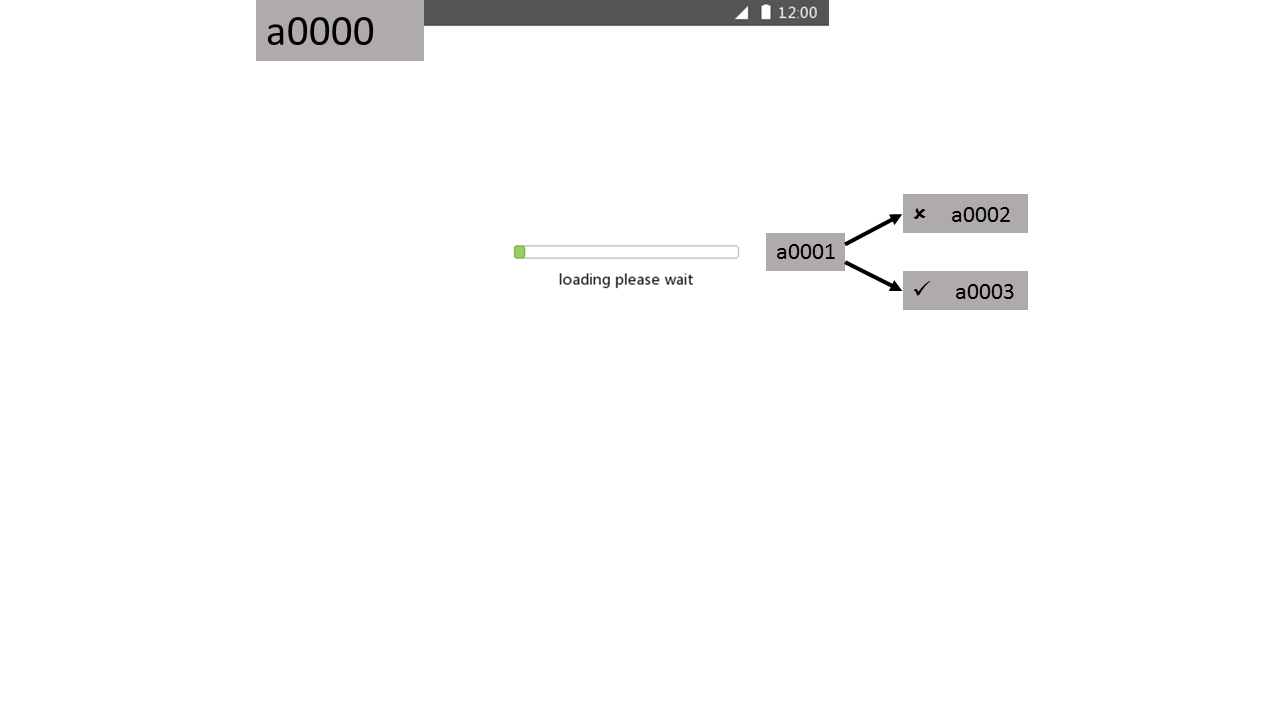
\includegraphics[width=\linewidth,height=\textheight,keepaspectratio]{Dialoge/a0000}
\caption{Starten der Software}
\end{figure}
\FloatBarrier

\subsubsection{Dialog a0100 – Startseite}
\begin{figure}[!htbp]
\centering
\noindent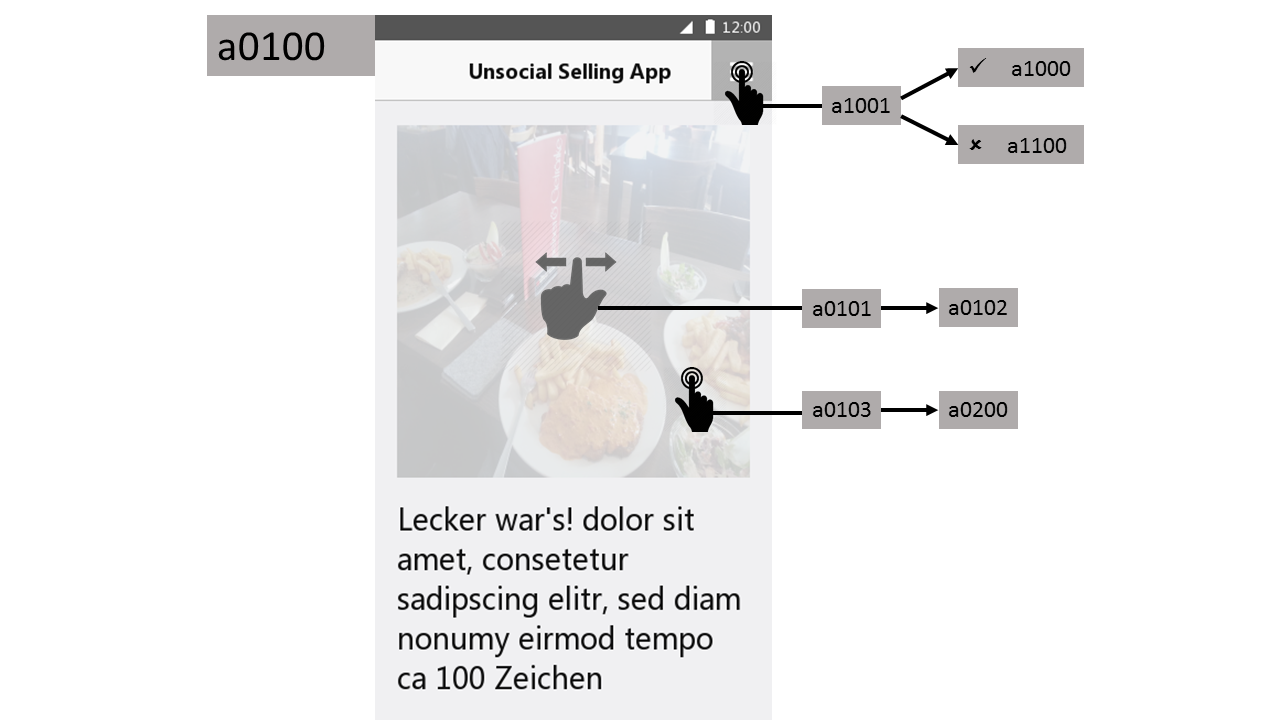
\includegraphics[width=\linewidth,height=\textheight,keepaspectratio]{Dialoge/a0100}
\caption{Startseite}
\end{figure}
\FloatBarrier

\subsubsection{Dialog a0200 – Detailansicht}
\begin{figure}[!htbp]
\centering
\noindent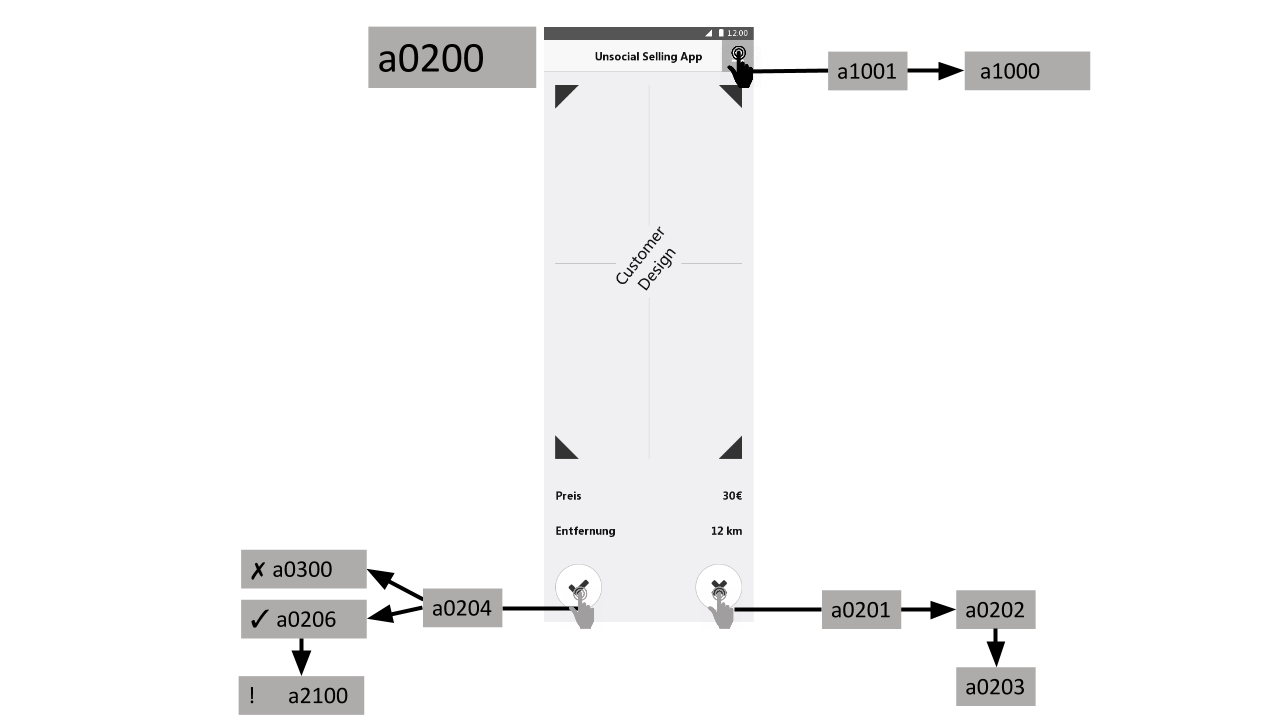
\includegraphics[width=\linewidth,height=\textheight,keepaspectratio]{Dialoge/a0200}
\caption{Detailansicht}
\end{figure}
\FloatBarrier

\subsubsection{Dialog a0300 – Einloggen}
\begin{figure}[!htbp]
\centering
\noindent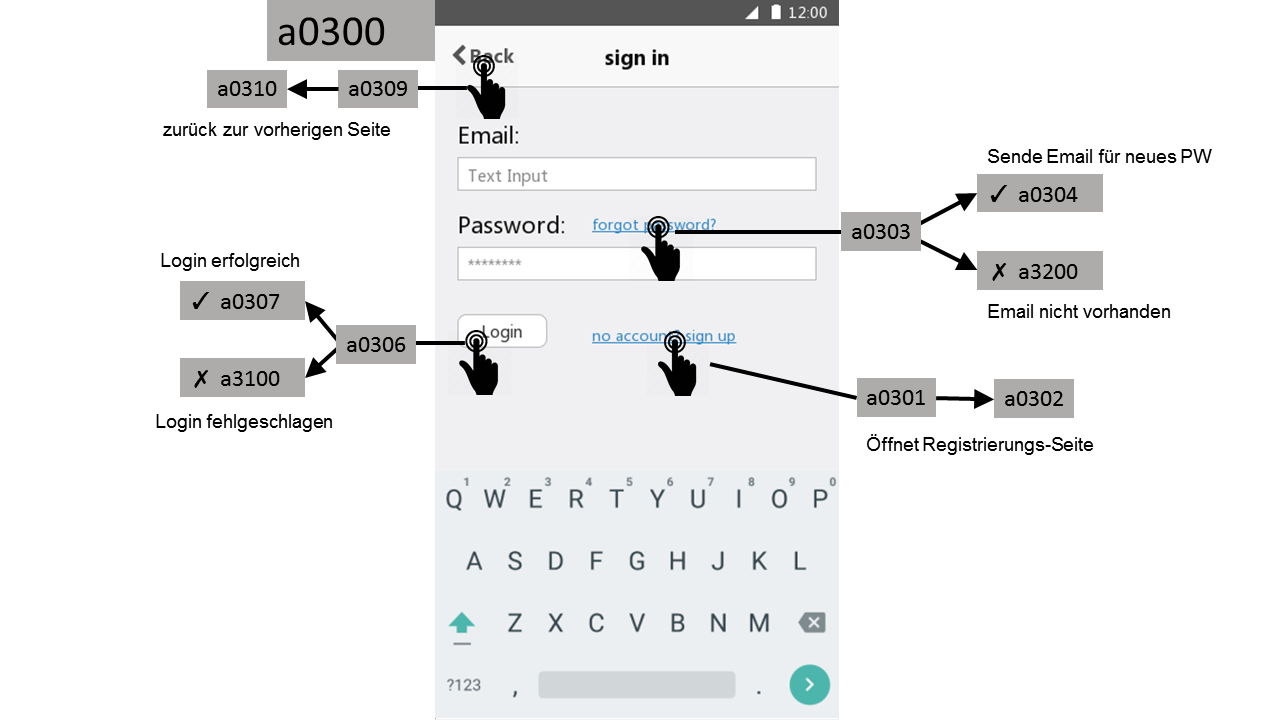
\includegraphics[width=\linewidth,height=\textheight,keepaspectratio]{Dialoge/a0300}
\caption{Einloggen}
\end{figure}
\FloatBarrier

\subsubsection{Dialog a0400 – Registrieren}
\begin{figure}[!htbp]
\centering
\noindent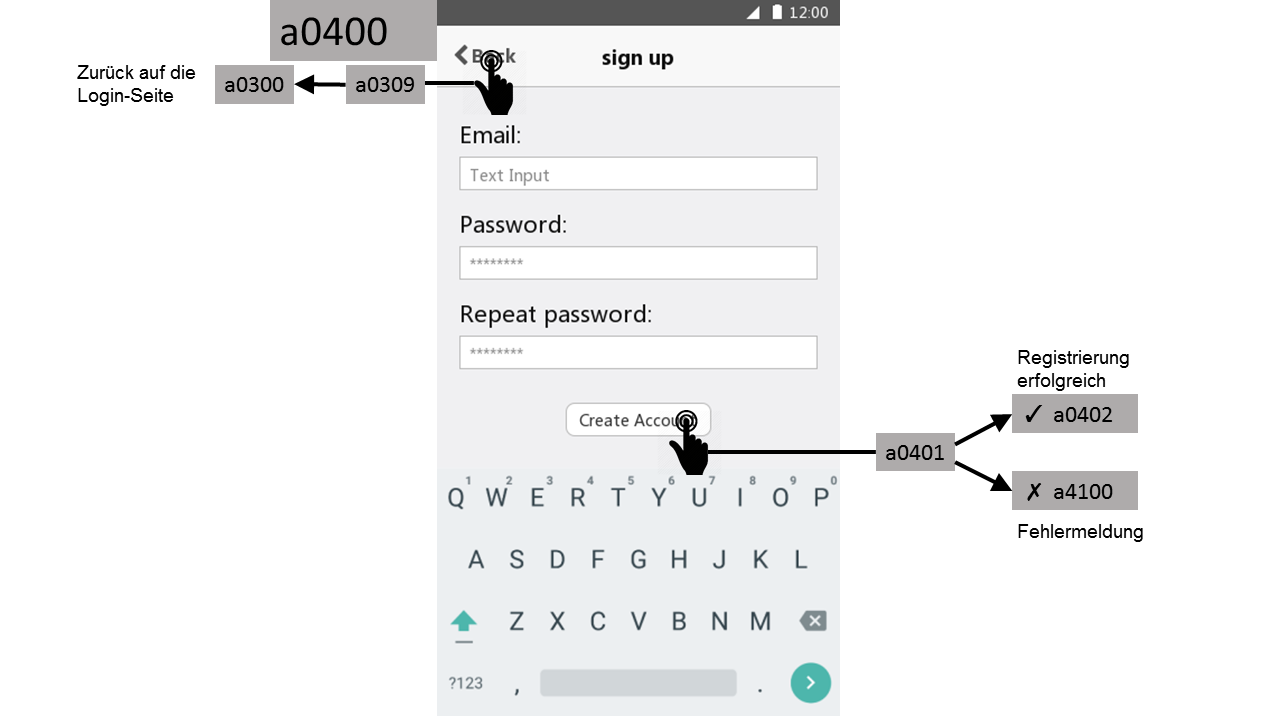
\includegraphics[width=\linewidth,height=\textheight,keepaspectratio]{Dialoge/a0400}
\caption{Registrieren}
\end{figure}
\FloatBarrier

\subsubsection{Dialog a0600 – Interessen Liste}
\begin{figure}[!htbp]
\centering
\noindent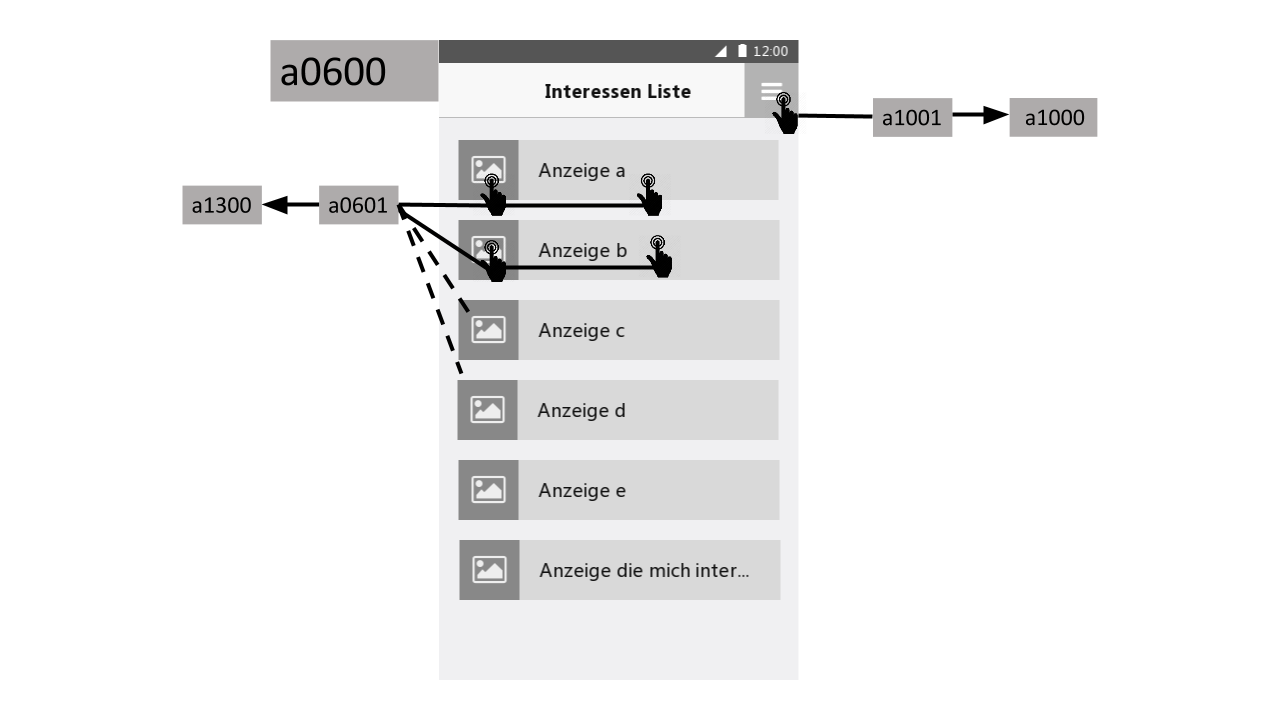
\includegraphics[width=\linewidth,height=\textheight,keepaspectratio]{Dialoge/a0600}
\caption{Interessen Liste}
\end{figure}
\FloatBarrier

\subsubsection{Dialog a0700 – Einstellungen}
\begin{figure}[!htbp]
\centering
\noindent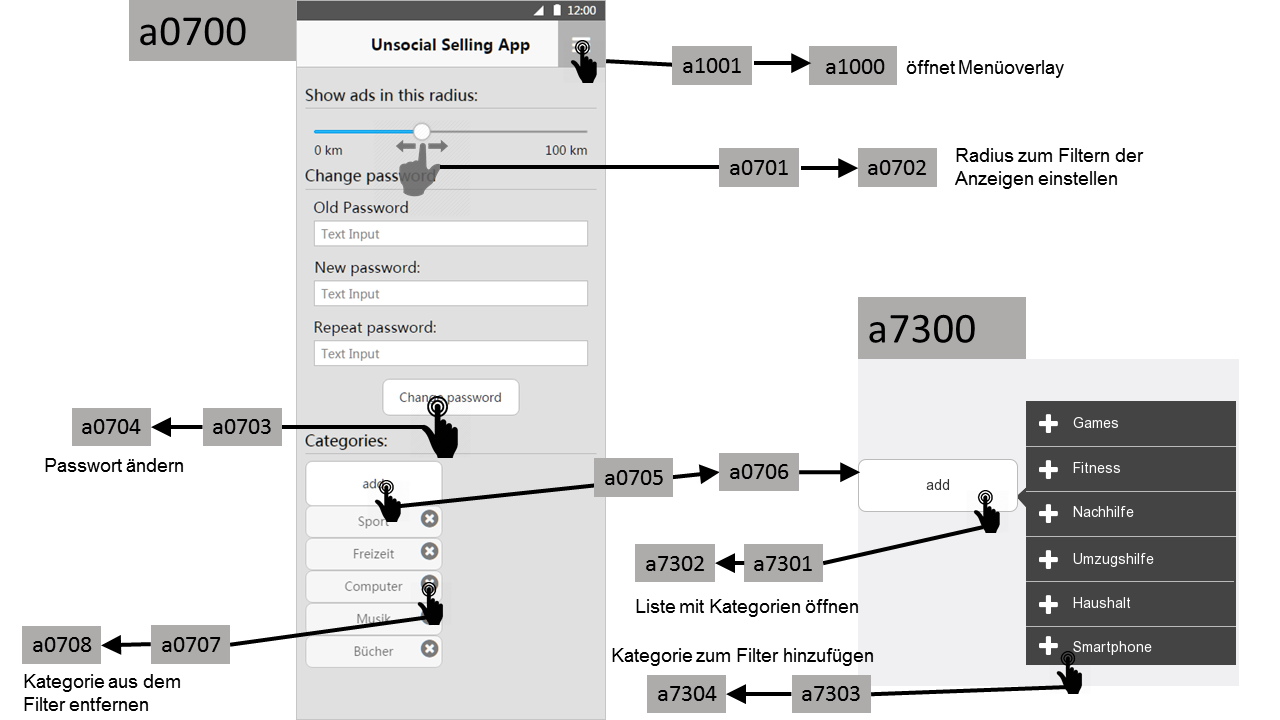
\includegraphics[width=\linewidth,height=\textheight,keepaspectratio]{Dialoge/a0700}
\caption{Einstellungen}
\end{figure}
\FloatBarrier

\subsubsection{Dialog a0800 – eingestellte Anzeigen Liste}
\begin{figure}[!htbp]
\centering
\noindent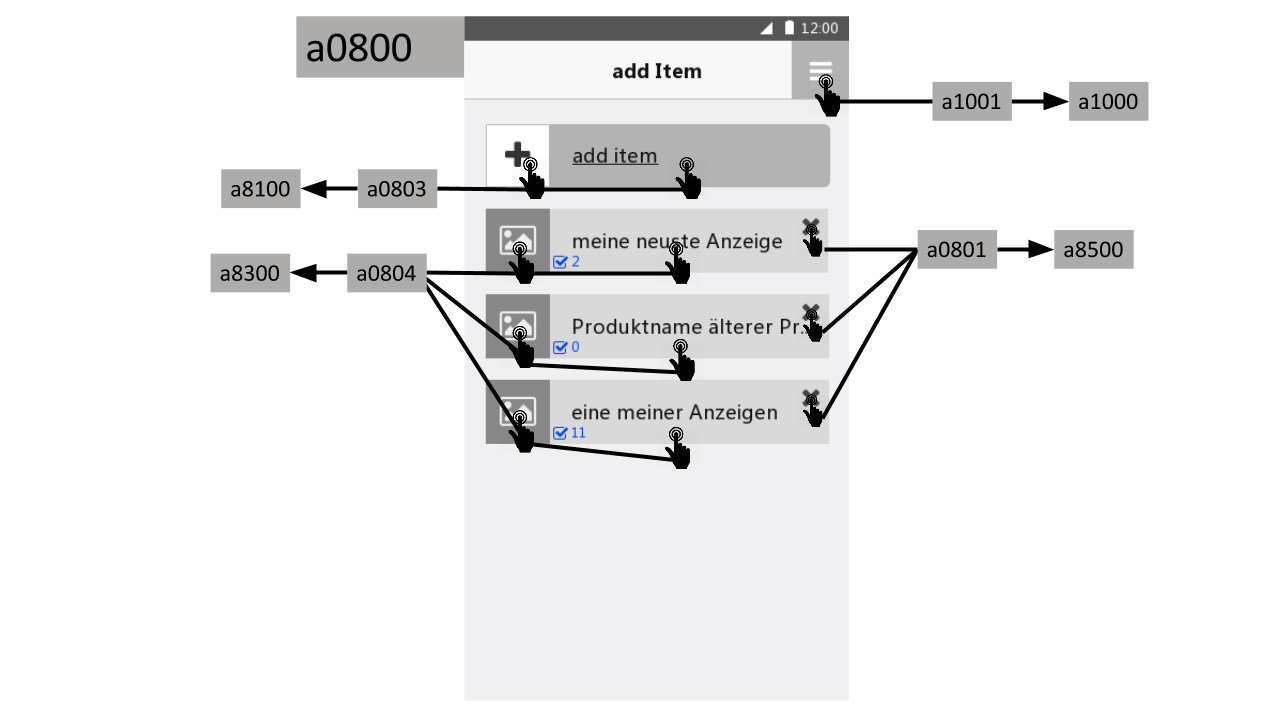
\includegraphics[width=\linewidth,height=\textheight,keepaspectratio]{Dialoge/a0800}
\caption{eingestellte Anzeigen Liste}
\end{figure}
\FloatBarrier

\subsubsection{Dialog a8100 – neue Anzeige einstellen }
\begin{figure}[!htbp]
\centering
\noindent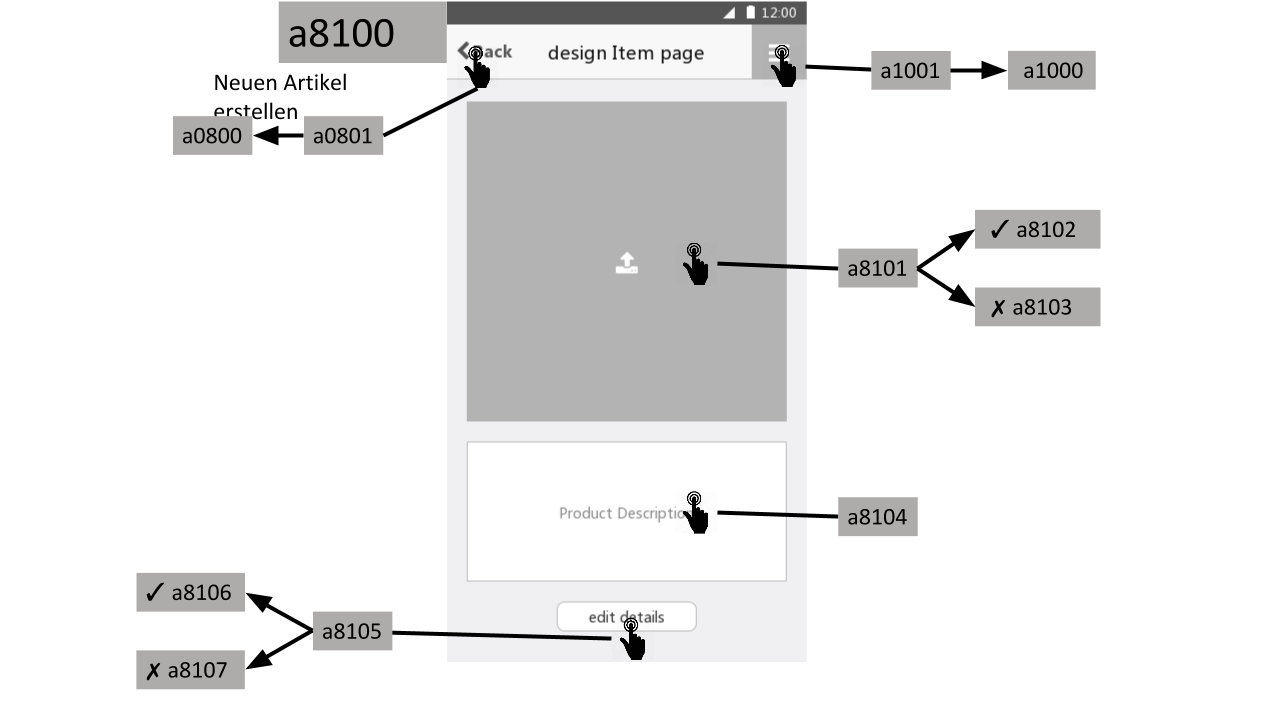
\includegraphics[width=\linewidth,height=\textheight,keepaspectratio]{Dialoge/a8100}
\caption{neue Anzeige einstellen}
\end{figure}
\FloatBarrier

\subsubsection{Dialog a8300 – Detailansicht editieren}
\begin{figure}[!htbp]
\centering
\noindent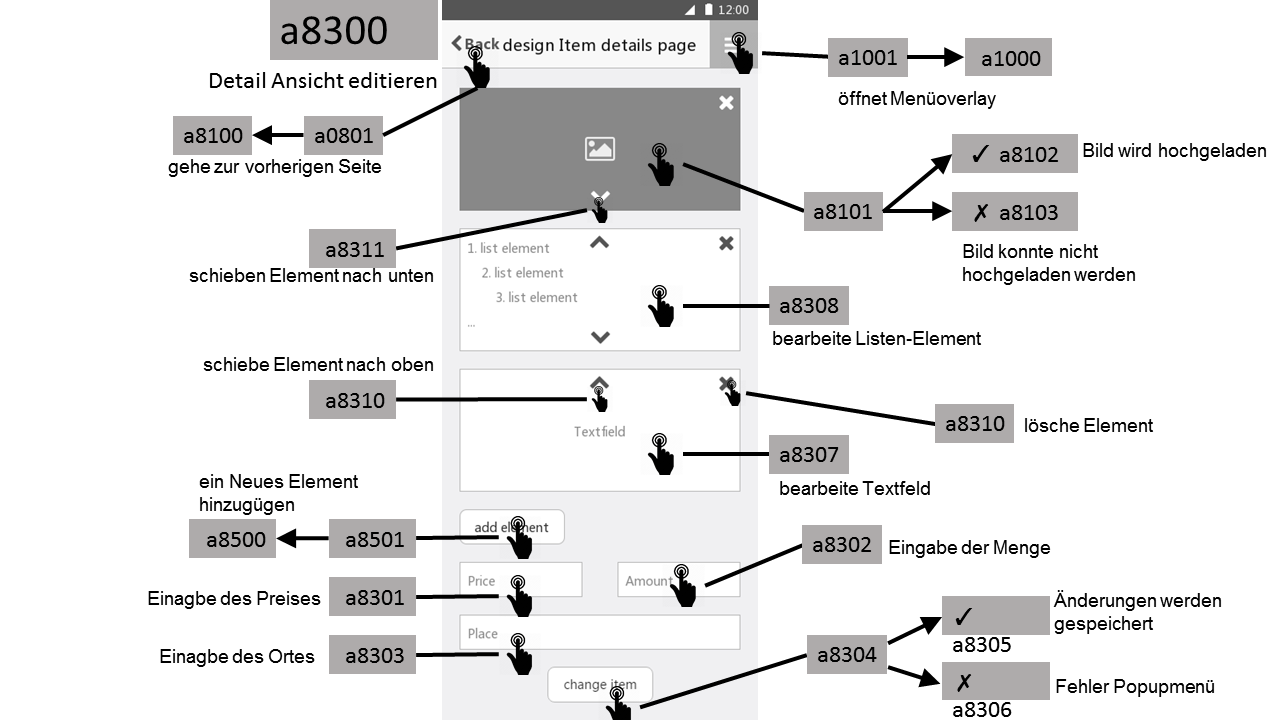
\includegraphics[width=\linewidth,height=\textheight,keepaspectratio]{Dialoge/a8300}
\caption{Detailansicht editieren}
\end{figure}
\FloatBarrier

\subsubsection{Dialog a8400 – Detailansicht designen}
\begin{figure}[!htbp]
\centering
\noindent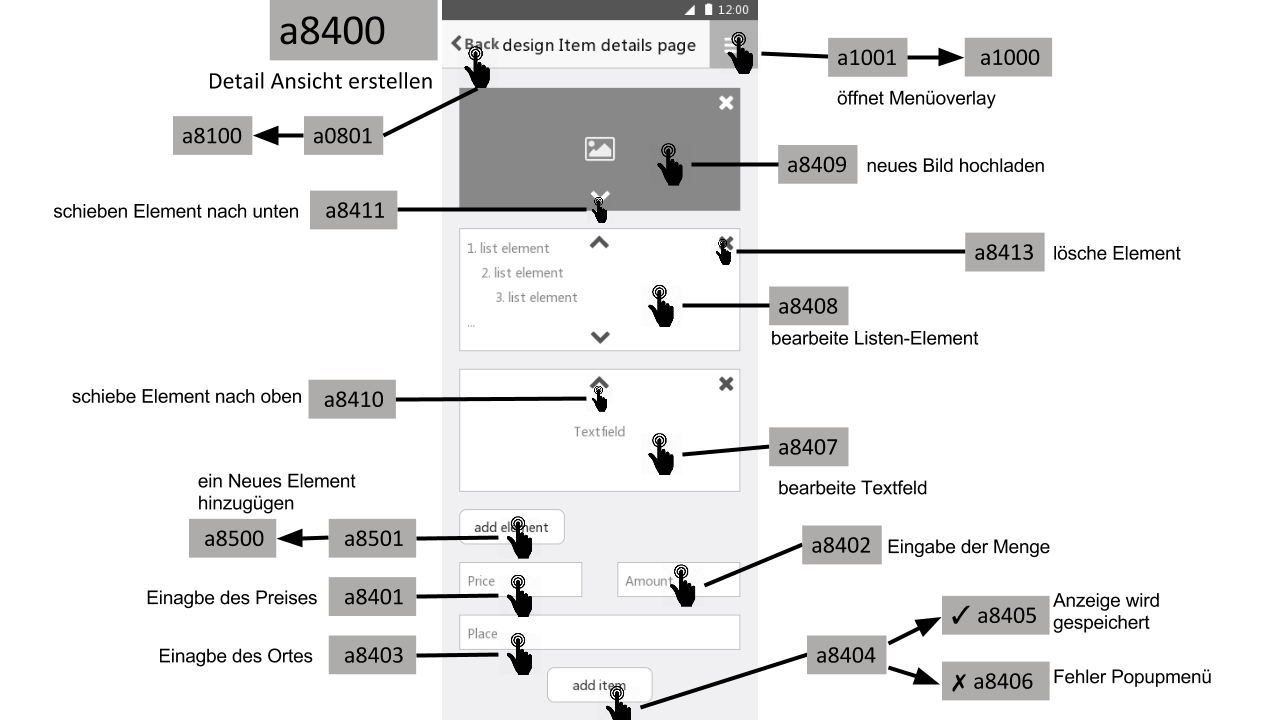
\includegraphics[width=\linewidth,height=\textheight,keepaspectratio]{Dialoge/a8400}
\caption{Detailansicht designen}
\end{figure}
\FloatBarrier

\subsubsection{Dialog a8500 – „add Item“ Menü}
\begin{figure}[!htbp]
\centering
\noindent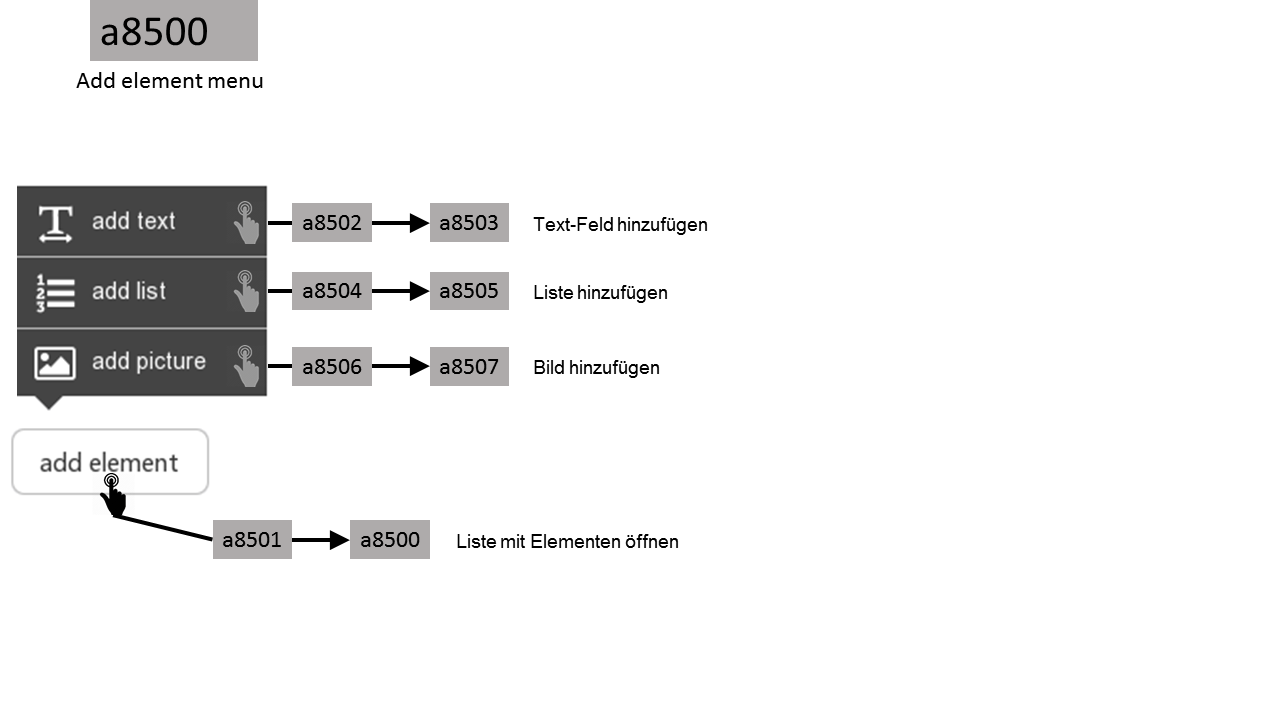
\includegraphics[width=\linewidth,height=\textheight,keepaspectratio]{Dialoge/a8500}
\caption{„add Item“ Menü}
\end{figure}
\FloatBarrier

\subsubsection{Dialog a1000 – Menü}
\begin{figure}[!htbp]
\centering
\noindent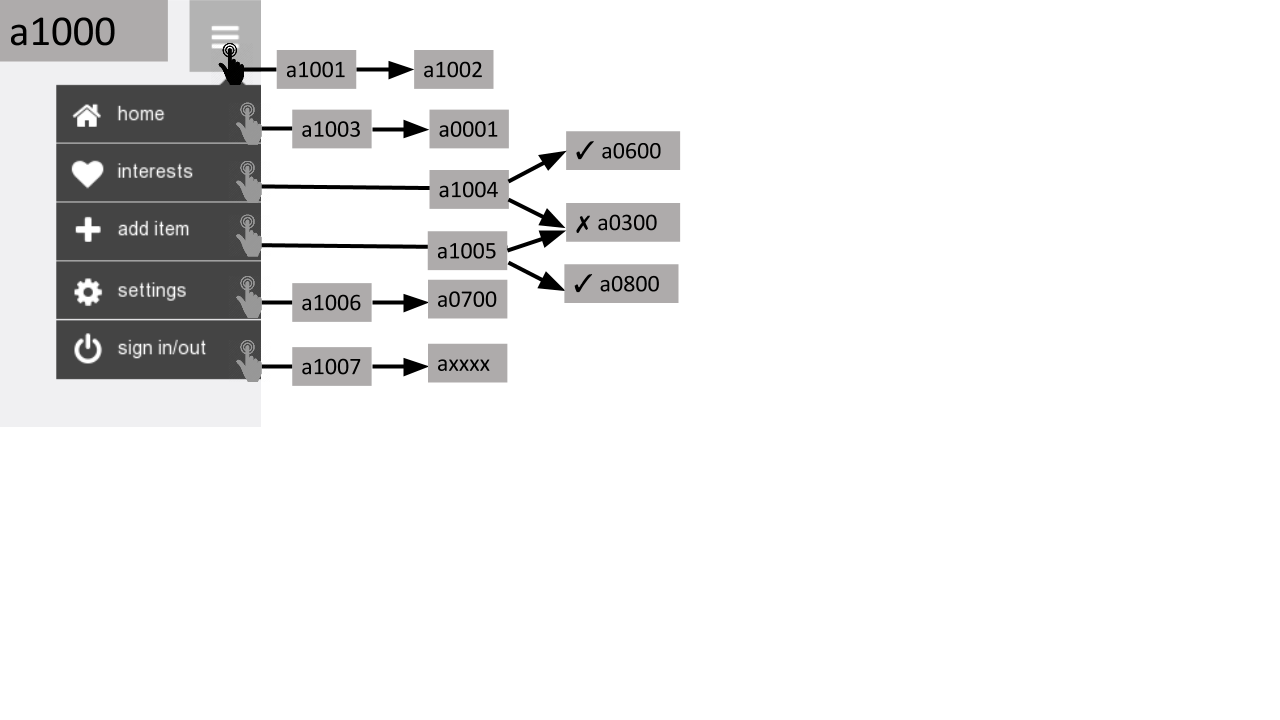
\includegraphics[width=\linewidth,height=\textheight,keepaspectratio]{Dialoge/a1000}
\caption{Menü}
\end{figure}
\FloatBarrier


\section{Produktdaten}
\subsection{Mengengerüst}
Anforderungen aufgrund des Mengengerüsts. 

\subsubsection*{MENGE\_001 - Benutzeranzahl}
\begin{itemize}
	\item Mit der Software müssen mindestens 300 Personen arbeiten können. 
	\item Jedem Benutzer muss mindestens 20 MB Speicherplatz zur Verfügung gestellt werden. 
\end{itemize}

\subsubsection*{MENGE\_002 - Anzahl der Vorgänge }
\begin{itemize}
	\item Pro Tag müssen mindestens 100 Anzeigen erstellt werden können. 
	\item Pro Tag müssen mindestens 1000 Anzeigen angesehen werden können.
\end{itemize}


\subsection{Vorgaben für Hardware, Software, Schnittstellen}
Die Applikation wird in zwei Teile unterteilt.
Ein Teil ist die SQL-Server, der andere die Client Applikation, die auf allen Endgeräten installiert wird.

\subsubsection*{Server}
Auf dem Server werden die Benutzerdaten, Verkaufsdaten in einer Datenbank gespeichert.
Der Server muss über folgende Ausstattungsmerkmale verfügen:
\begin{itemize}
	\item MySQL 10.0.17-MariaDB
	\item OS: Linux oder Windows
	\item HD mindestens 10 GB
	\item 2 GB RAM
\end{itemize}

\subsubsection*{Client}
Der Client muss eine ständige Verbindung zum Internet besitzen.
Die Applikation muss auf Android, Windows Phone, Windows und iOS lauffähig sein. Optimierung für genaue Modelle ist nicht gefordert.
Die App benötigt maximal 50MB an Speicherplatz. 


\section{Produktleistungen}
\subsection{Performance}


\section{Qualitätsanforderungen}
\subsection{Bedienbarkeit, Zuverlässigkeit, Effizienz}
Die Applikation muss unter den aktuellen Versionen von Android, iOS und Windows Phone lauffähig sein.
Es muss außerdem eine Applikation für Desktop-PCs geben.

\subsubsection*{Anforderung an die Zuverlässigkeit}
Die Konsistenz der Datenbank, muss jederzeit gewährleistet werden.



\end{document}